\section{Summary of Proteome Data: Experimental Details}
\label{sec:SI_exp_summary}

Here we provide a brief summary of the experiments behind each proteomic data
sets. The purpose of this section is to better identify the steps taken by the
authors to arrive at absolute protein abundances. In the following section
(Section~\nameref{sec:SI_data_summary}) we will then provide a summary of the
final protein abundance measurements that were used for in the main text. Table
\ref{table:datasets} provides an overview of the main data sets that we
considered. These are predominately mass spectrometry-based, with the exception
of the work from Li \textit{et al.} (2014) which used ribosomal profiling, and
the fluorescence-based counting done in Taniguchi \textit{et al.} (2010).

\begin{table}[bt]
\caption{\label{tab:datasets}Overview of proteomic data sets.}
% Use "S" column identifier to align on decimal point
\begin{tabular}{l l l }
\toprule
Author & Method & Reported Quantity \\
\midrule
Taniguchi \textit{et al.} (2010)  & YFP-fusion, cell fluorescence    & fg/copies per cell      \\
Valgepea \textit{et al.} (2012)   & mass spectrometry                & fg/copies per cell      \\
Peebo \textit{et al.} (2014)      & mass spectrometry                & fg/copies per fl        \\
Li \textit{et al.} (2014)         & ribosomal profiling              & fg/copies per cell $^a$ \\
Soufi \textit{et al.} (2015)      & mass spectrometry                & fg/copies per cell      \\
Schmidt \textit{et al.} (2016)    & mass spectrometry                & fg/copies per cell $^b$ \\
\bottomrule
\end{tabular}

\medskip
a. The reported values assume that the proteins are long-lived compared to the
generation time but are unable to account for post-translational modifications
that may alter absolute protein abundances.
\\
b. This mass spectrometry approach differs substantially from the others since
in addition to the relative proteome-wide abundance measurements, the authors
performed absolute quantification of 41 proteins across all growth conditions
(see Section~\nameref{sec:SI_schmidt} for more details on this).
\end{table}

\subsection{Fluorescence based measurements}
In the work of \cite{taniguchi2010}, the authors used a chromosomal YFP fusion
library where individual strains have a specific gene tagged with a YFP-coding
sequence. 1018 of 1400 attempted strains were used in their work. For each
strain, a fluorescence microscope was used to collect cellular YFP intensities.
Through automated image analysis, the authors normalized intensity measurments
by cell size to account for the change in size and expression variability across
the cell cycle. YFP intensities were also corrected for cellular
autofluorescence, and final absolute protein levels were determined by a
calibration with single-molecule fluorescence intensities, performed seperately
using a purified YFP solution.

\subsection{Ribosomal profiling measurements}
The work of \cite{li2014} takes a sequencing based approach to estimate protein
abundance. Ribsomal profiling, which refers to the deep sequencing of
ribosome-protected mRNA fragments, provides a quantitative measurement of the
protein synthesis rate.  As long as the protein life-time is long relative to
the cell doubling time, it is possible to  also estimate absolute protein copy
numbers.

To perform ribosomal profiling, ribosome-protected mRNA is extracted from cell
lysate  and selected on a denaturing polyacrylamide gel, and sequences are
obtained by deep sequencing (15–45 nt long fragments collected and sequenced  by
using an Illumina HiSeq 2000 in \cite{li2014}). Counts of ribosome footprints
from the sequencing data are corrected empirically for position-dependent biases
in ribosomal density across each gene, as well as dependencies on specific
sequences including the Shine-Dalgarno sequence. These data-corrected ribosome
densities represent relative protein synthesis rates.

Absolute protein synthesis rates are obtained by multiplying the relative rates
by the total cellular protein per cell. The total protein  per unit volume  was
determined with the Lowry method to quantify total protein, calibrated against
bovine serum albumin (BSA). By counting colony-forming units following serial
dilution of their cell cultures, they then calculated the total protein per
cell. The absolute protein synthesis rate has units of  proteins per generation,
and for stable proteins will also correspond to the protein  copy number per
cell.

\subsection{Mass spectrometry measurements}

Perhaps not surprisingly, the data is predominantly mass spectrometry based. This is
largely due to tremendous improvements in the sensitivity of mass spectrometers,
as well as improvements in sample preparation and data analysis
pipelines. It is now a relatively routine task to extract protein from a cell
and quantify the majority of proteins by shotgun proteomics. In general, this
involved lysing cells, enzymatically digesting the proteins into short peptide
fragments, and then introducing them into the mass spectrometer (commonly
employing liquid chromatography and electrospray ionization), which itself can
have multiple rounds of detection and further fragmentation of the peptides.

Most quantitative experiments rely on labeling protein with stable isotopes,
which allow multiple samples to be measured simultaneously by the mass
spectrometer. By combining samples of known total protein abundance (i.e. one
sample of interest, and one reference), it is possible to determine relative
protein abundances. With relative protein abundances in hand, absolute protein
abundances can be estimated following the same approach used above for ribosomal
profiling, which is to multiply each relative abundance measurement by the total
cellular protein per cell. This is the approach taken by \cite{valgepea2013} and
\cite{peebo2015}, with relative protein abundances determined based on the
relative peptide intensities (label free quantification 'LFQ' intensities). For
the data of \cite{valgepea2013}, total protein per cell was determined by
measuring  total protein by the Lowry method, and counting colony-forming units
following serial dilution. For the data from   \cite{peebo2015}, the authors did
not determine  cell quantities and instead report the cellular protein
abundances in protein per unit  volume by assuming a mass density of 1.1 g/ml,
with a 30\% dry mass fraction.

A key distinction in the mass spectrometry work of \cite{schmidt2016} is that in
addition to determining relative abundance, they performed absolute
quantification of  41 enzymes covering over four orders of magnitude in cellular
abundance. Here,  a synthetic peptide was generated for each of the 41 proteins,
doped into each protein sample, and used to provide an calibration between
measured mass spectrometry intensities and absolute protein abundances. These
absolute measurements, determined for every growth condition considered in their
work,   were then used as a calibration curve to convert proteomic-wide relative
abundances into  absolute protein abundance per cell. A more extensive
discussion of the \cite{schmidt2016} data set can be found in Section
\nameref{sec:SI_schmidt} .

\section{Summary of Proteomic Data}
\label{sec:SI_data_summary}

In \FIG{upset} we show the coverage and overlap of all proteins quantified
across each data set using an UpSet diagram \citep{Lex2014}.


\begin{figure*}
    \centering{
        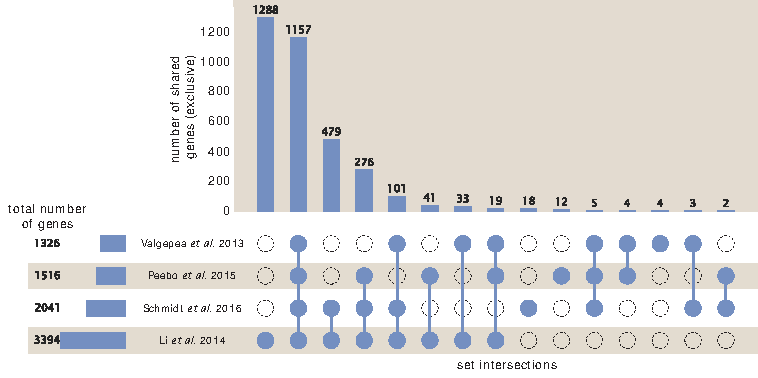
\includegraphics{SI_figs/dataset_upset_diagram.pdf}
        \caption{\textbf{Comparison of proteomic coverage across different data sets.} } \label{fig:upset}
    }
\end{figure*}


\begin{figure*}
    \centering{
        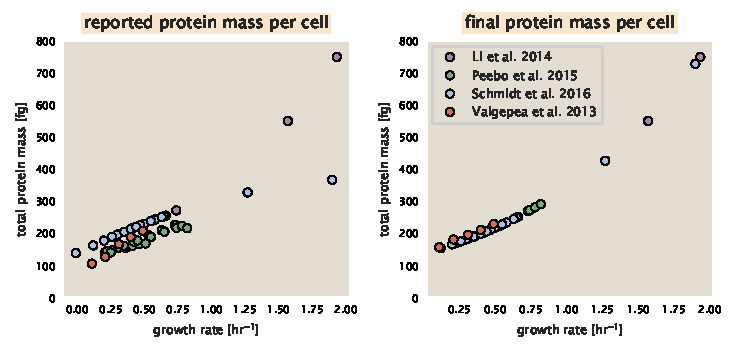
\includegraphics{SI_figs/dataset_corrections.pdf}
        \caption{\textbf{Summary of the growth-rate dependent total protein abundance for each data set.} } \label{fig:total_protein_final}
    }
\end{figure*}
